% !TEX root = ../main.tex
\chapter{Spellcasting} \label{ch::spellcasting}

% \subparagraph{Eldremry} % indigo tide, earth, cross
%     \textbf{TODO}.
%     Born from the indigo tide, Eldremry focuses on reshaping earth itself.
%     Spells from this doctrine were used by Hairuus to create their island cities, but all traces of it were lost along with the nation.
%     SCHOOLS: Geomancy

% \subparagraph{Sigaldry} % silver tide, metal, split
%     \textbf{TODO}.
%     Born from the silver tide, this doctrine focuses on evoking effects from written words and special symbols.
%     Sigaldry spells are highly sought after by blacksmiths, as runes from this doctrine are known to infuse strong effects on metal objects.
%     SCHOOLS: Guentsue, Mevthan, Shazdrala

% \subparagraph{Alchemy} % blue tide, water, drill
%     \textbf{TODO}.
%     Born of the blue tide, this doctrine focuses on manipulating the energy contained in each living being.
%     Some schools focus on bringing out potent effects from food and drinks, while others enhance or impair a creature's ability directly.
%     SCHOOLS: Qerestad, Cthai'khas (fleshshaping), warchanting

% \subparagraph{Thaumaturgy} % gold tide, wood, crush
%     \textbf{TODO}.
%     Born from the gold tide, this doctrine focuses on the power of words, both spoken and written.
%     Thaumaturges use the power of their own voice to issue irresistible commands or veil one's eyes with insurmountable illusions.
%     SCHOOLS: Dremshamad (Written contracts and stuff), The Voice, Mephetis' thaumaturgy

% TODO. Missing spellcasting doctrines:
% Uldammy (white tide, wind, void) - focuses on changing the wind (like dentrala), lack of stuff (like Darkness) and shit.
% Rashid - manipulates the connection between tides and bringing in the essence of them.
% NOTE. The spellcasting focus for Rhashid and any tidal magic is your qualar.
% NOTE. PHARIKA SHIT. All weapons have some poison in them. Critical hits gain a damage bonus equal to double your Wisdom modifier.

% TODO. Explain rules.
% !TEX root = ../main.tex
\section{Spellcasting Rules} \label{sec::spellcastingrules}
\subsection*{Spellcasting Doctrines}
    There exist five spellcasting doctrines in Yuadrem, each related to a tide.
    Many schools belong to each doctrine, but all are related at heart.

    In general, casting a spell requires certain conditions to be met.
    These conditions depend on the spell itself, but can be categorized by the spellcasting doctrine to which they belong.
    Each doctrine and its method for casting spells is detailed in the following sections.

    In addition, each doctrine's spells are separated into three categories, each associated to conditions from the doctrine.
    For example, sympathists have three methods for tethering: heat, electric, and similarity links.
    When you take the spellcaster feat and choose a doctrine, select two of these categories.
    You learn the mediums associated to the categories, and you can learn any of the basic spells from those categories.
    To learn advanced spells, you need to take the \textbf{Upgraded Spellcasting} major character advancement (page \pageref{feat::upgradedspellcasting}).

\subsection*{Spellcasting Ability}
    When you take the spellcaster feat, you decide a spellcasting ability, which can be Intelligence, Wisdom, or Charisma.
    This choice reflects your medium for casting spells: Conceptualization for Intelligence, volition for Wisdom, and empathy for Charisma.

    You use this ability score whenever a spell refers to your spellcasting ability.
    In addition, you use its modifier when setting the saving throw DC for a spell you cast and when making an attack roll with one.

    \textbf{Spell save DC} = 8 + your spellcasting proficiency bonus + your chosen ability modifier

    \textbf{Spell attack modifier} = your spellcasting proficiency bonus + your chosen ability modifier

    After taking the spellcaster feat, your spellcasting proficiency bonus is +2.
    You can increase this modifier further by taking the \textbf{Avid Caster} feat (see page \pageref{feat::avidcaster}).

\subsection*{Known Spells}
    As a user of magic, you know a number of spells which you can use in any scenario you find appropiate.
    The maximum number of spells you can have prepared at a time is equal to your spellcasting ability modifier + half your level (rounded down).
    If you add a new spell when you already have the maximum number of spells prepared, you forget one spell of your choice.
    To keep these spells available, you can use a spellbook (see page \pageref{item::spellbook}).

    When you take the \textbf{Spellcaster} feat (page \pageref{feat::spellcaster}), you gain access to three mediums and two spells.
    Two of the mediums and one spell are of your choice within your chosen doctrine, and the other medium and spell comes from the spellcasting school of your choice.
    The spell associated to your school does not count towards your number of known spells.

    When you take the \textbf{Spellcaster} feat you only gain access to basic spells, as marked in the \textbf{Basic Spells} section (page \pageref{sec::basicspells}).
    By taking the \textbf{Upgraded Spellcasting} major character advancement (page \pageref{mca::upgradedspellcasting}), showing your commitment to your school, you gain access to advanced spells, which can be seen in the \textbf{Advanced Spells} section (page \pageref{sec::advancedspells}).

    You can learn one new spell as part of a long rest.
    This spell must belong to a spellcasting doctrine available to you and be related to your mediums.

\subsection*{Spell Points}
    Your character uses spell points to fuel spells.
    Each spell has a point cost based on its strength, which is detailed in the spell's description.
    Mediums don't require spell points to be cast.
    You recover all spent spell points after a short rest.

    The number of spell points you have to spend is based on your level, as shown in the spellcasting ability table.
    In addition, you can gain access to more spell points by taking the \textbf{Upgraded Spellcasting} major character advancement.

    \begin{DndTable}[width=\linewidth, header=Spellcasting Ability]{lllll}
        \textbf{Level} &  \textbf{Spell Points} & \hspace{0.5cm} & \textbf{Level} & \textbf{Spell Points} \\
         1st &     2 &  & 11th &    36 \\
         2nd &     3 &  & 12th &    38 \\
         3rd &     7 &  & 13th &    41 \\
         4th &     8 &  & 14th &    44 \\
         5th &    13 &  & 15th &    47 \\
         6th &    16 &  & 16th &    50 \\
         7th &    19 &  & 17th &    53 \\
         8th &    22 &  & 18th &    57 \\
         9th &    28 &  & 19th &    61 \\
        10th &    32 &  & 20th &    66
    \end{DndTable}

    % \thispagestyle{empty} % Remove footer so that it doesn't clash with the image.
    % \begin{tikzpicture}[remember picture,overlay]
    %     \node[anchor=south, yshift=-0.10cm] at (current page.south) {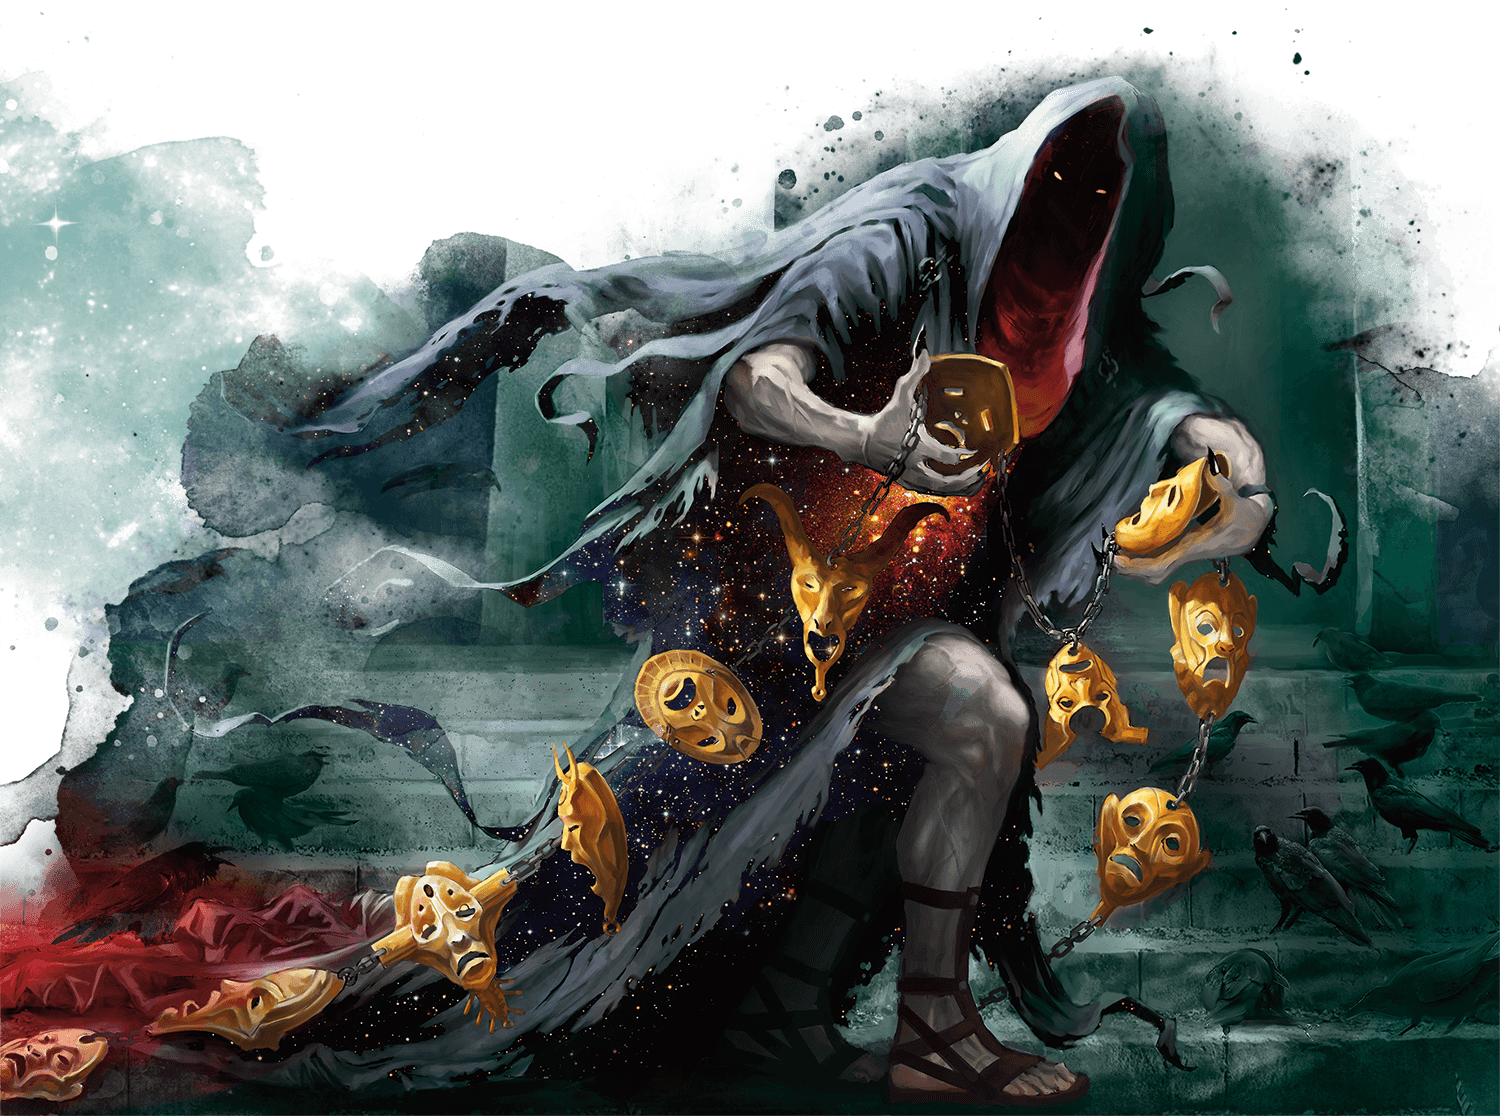
\includegraphics[width=\pdfpagewidth]{07spellcasting/img/10erebos.png}};
    % \end{tikzpicture}

\newpage
% NOTE. I will probably end up filling this space with a corner image.

% !TEX root = ../main.tex
\section{Sympathy} \label{sec::sympathy}
% Red tide, fire, explode
% SCHOOLS: Queish, Eljur, !Flamespeaking

Born from the red tide, the sympathy doctrine focuses on tethering links, the exchange of properties, and the redirection of energy.
Oft called Sympathists, sympathy spellcasters establish sympathetic links of different kinds between objects and creatures, altering the world around them through these.

Sympathists manifest effects on the world via sympathetic links.
These links can be of three natures: heat, electric, and similarity.

\subparagraph{Heat Link}
    (see page \pageref{medium::ember}).
    Sympathy spellcasters can quickly produce great surges of energy around them, but these are useless without a spark to ignite them.
    Heat links are floating embers which act as these sparks.

\subparagraph{Electric Link}
    (see page \pageref{medium::charge}).
    In contrast with fire, sympathists don't require a spark to manifest energy in its most pure form: electricity.
    Nonetheless, without a charge to guide lightning, it just takes the shortest route towards the ground.
    Sympathists use electric links to apply these charges to creatures and objects around them, enabling them to direct lightning at foes and allies alike.

\subparagraph{Similarity Link}
    (see page \pageref{medium::tether}).
    Unlike other sympathetic mediums, similarity links connect creatures and objects to exchange properties between them.
    A sympathist can tether these links to, for example, increase the weight of a creature, change its form, levitate it, etc.

\subsection*{Flamespeaking} \label{ssec::flamespeaking}
    \textit{I see your future, mantled in ash.}

    The seers of Viphoger are said to be blessed by the gods, granted special sight that sees past our world, into the stars of Nyx and beyond.
    Even novice seers are able to glimpse the weave of fate, seeing the connections of destiny that bind us all.
    With proper training, years of practice, and a bit of intuition, the best soothsayers can foretell every possible future, not just those most likely.

    Flamespeakers are special seers, blessed by Purphoros, god of the forge.
    Through the god's divine power, they are able to see portents in the curl of smoke, the flicker of flames, and the patterns of ash.

    When you choose this spellcasting school, you learn the \textbf{Firetrap} heat link (see page \pageref{medium::firetrap}), as well as the \textbf{Screaming Bead} spell (see page \pageref{spell::screamingbead}).
    Neither the medium nor the spell count towards your known mediums and spells.

\pagebreak

    % \subsubsection{Flickering Future}
    %     With the exception of those blessed by Keranos, god of insight, or Klothys, god of destiny, the powers of a seer depend very little on which god they've received their sight from.
    %     The only variation is often in what they are able to see from their future --- for example, seers blessed by Erebos are usually haunted by visions of death, while those blessed by Nylea might know exactly when and where to find the quarry of their hunt.
    %
    %     Most seers receive their portents by sight, in moments when their eyes look beyond, to the weave of fate, and follow the tangled lines therein.
    %     The flamespeakers of Purphoros are different in that they are unable to see the weave directly, but instead view it in every spark and ember of fire.
    %     For them, fire and destiny are inextricable, one and the same, with the weave of destiny imprinted onto a fundamental force of the world.
    %
    % \subsubsection{Twist the Lines}
    %     While the method with which they view the future is novel, what truly sets the flamespeakers apart is their ability to twist and tangle the pieces of the weave that they can see.
    %     Like many of Purphoros' priests, the flamespeakers are vessels for the god's power, granting them control over fire in its many forms.
    %     But for the flamespeakers, control of fire means a control of destiny.
    %
    %     The flamespeakers are able to change the future as they see in the ashes.
    %     It requires great effort on their part, and the changes are rarely more than minor, but it can be done all the same.
    %     For this reason, the flamespeakers are highly sought after, especially by those who have been informed of a terrible fate destined to befall themselves or a loved one.

% !TEX root = ../main.tex
\section{Sigaldry} \label{sec::sigaldry}
\textbf{TODO}.
\newpage

% !TEX root = ../main.tex
\section{Alchemy} \label{sec::alchemy}
\textbf{TODO}.
\newpage

% Zuan can be moved up to 4 meters as a free action.

% !TEX root = ../main.tex
\section{Thaumaturgy} \label{sec::thaumaturgy}
\textbf{TODO}.
\newpage


% TODO. ! Thaumaturgy spellcasting school.
% TODO. ! Tortle alchemy-like chemistry, based on cooking to enhance effect of drugs and potions.
% TODO. ! Poison and alchemy stuff from followers of Pharika.
% TODO. ! Warchanting - using drugs and rituals to enhance rage in the name of Mogis.
    % Rage burns a spell point each turn while its activated, and other effects can use more spell points.
    % Rage has all the normal effects from the barbarian class.
    % lv 2: burn one additional spell point to gain one action during your turn.
    % lv 3: burn two spell points to ignore the multiple attack penalty while raging.

    % Bloodhorn Minotaurs
    % Named for their blood-caked horns, the Bloodhorn minotaurs have ragged claws to supplement their charges and gores. Gleeful in their brutality, they slaughter and devour any intruders they encounter in the badlands, and particularly value the bone marrow of young humans. They take pride in their overlarge, razor-sharp horns.

    % Felhide Minotaurs
    % The notoriously dour Felhide minotaurs are descended from the warlord Thyrogog of the Ashlands. The Theriad recounts the brute's defeat and the loss of his great axe, Goremaster. Viewing Thyrogog's defeat as a divine sign, the warlord's descendants retreated into the Ashlands.

    % Burial rites among the Felhide minotaurs involve devouring those who fell in battle, to remove their shame from memory and fuel the survivors' revenge. Should another scavenger reach a fallen Felhide before the rest of the band can eat the dead minotaur's remains, the minotaurs mobilize to track down as much of their dead comrade's body as possible.

    % Ragegore Minotaurs
    % Ragegore minotaurs are the most ferocious of their kind, deeply infected by the bloodlust of Mogis. Ragegores never withdraw from a battle, entering a frenzy of furious delight at the sight of an enemy's blood. While in the heat of battle, a Ragegore minotaur seems to feel no pain and barely notices wounds that would kill a human. Some Ragegores have been known to fall dead immediately at the cessation of battle, their life sustained only by their fury.
